\documentclass[border=0pt]{standalone}
\usepackage{amsmath,amssymb}
\usepackage{xcolor}
\usepackage{tikz}
\usetikzlibrary{arrows.meta,calc,decorations.pathreplacing,positioning,shapes.geometric,backgrounds}
\definecolor{c1}{RGB}{0,114,178}
\definecolor{c2}{RGB}{230,159,0}
\definecolor{c3}{RGB}{0,158,115}
\definecolor{cr}{RGB}{213,94,0}
\tikzset{every picture/.append style={show background rectangle,
    background rectangle/.style={fill=white}, inner frame sep=8pt}}
\newcommand{\roll}{\mathcal{R}}
\begin{document}
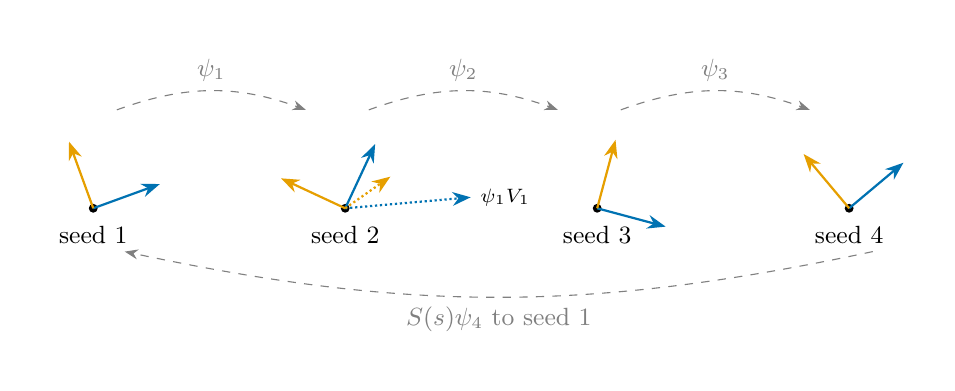
\begin{tikzpicture}[>=Stealth, scale=1.0]
    % seeds on a line
    \foreach \i in {1,...,4} {
      \coordinate (s\i) at ({3.2*(\i-1)}, 0);
      \fill (s\i) circle (1.6pt);
      \node[below=3pt, font=\small] at (s\i) {seed \i};
    }
    % orthonormal frames at every seed, before the step
    \foreach \i/\ang in {1/20, 2/65, 3/-15, 4/40} {
      \draw[->, c1, thick] (s\i) -- ++(\ang:0.9);
      \draw[->, c2, thick] (s\i) -- ++(\ang+90:0.9);
    }
    % the image of the frame of seed 1 at seed 2, and its orthonormalisation
    \draw[->, gray, dashed] ($(s1)+(0.3,1.25)$) to[bend left=20] node[above, font=\small] {$\psi_1$} ($(s2)+(-0.5,1.25)$);
    \draw[->, gray, dashed] ($(s2)+(0.3,1.25)$) to[bend left=20] node[above, font=\small] {$\psi_2$} ($(s3)+(-0.5,1.25)$);
    \draw[->, gray, dashed] ($(s3)+(0.3,1.25)$) to[bend left=20] node[above, font=\small] {$\psi_3$} ($(s4)+(-0.5,1.25)$);
    \draw[->, gray, dashed] ($(s4)+(0.3,-0.55)$) to[bend left=12] node[below, font=\small] {$S(s)\psi_4$ to seed 1} ($(s1)+(0.4,-0.55)$);
    % image at seed 2, skewed and stretched
    \draw[->, c1, densely dotted, thick] (s2) -- ++(5:1.6);
    \draw[->, c2, densely dotted, thick] (s2) -- ++(35:0.7);
    \node[font=\scriptsize, anchor=west] at ($(s2)+(5:1.6)$) {$\psi_1 V_1$};
  \end{tikzpicture}
\end{document}
